


\chapter{Mathematical Flexibility\label{ch:math}}
%-----------------------------------------------------------------------------

Introducing formal methods into a software engineering project causes a sharp increase in the up-front effort required to develop the software.  Appropriate mathematical theories must be developed, components must be formally specified by a software engineer trained in formal techniques, and verification conditions must be dispatched by a mathematician in a formal environment that eliminates the possibility of human error, possibly with the assistance of an automated proving tool.

While we argue that this cost is justified in critical or long-running deployments by a corresponding reduction in effort during the maintenance phase of the software lifecycle, it is undeniable that this remains a barrier for entry to many projects that could otherwise benefit from formal methods of quality assurance.  We hypothesized that a number of steps could be taken to reduce the real or percieved additional effort, as well as increase the corresponding long-term benefits.

%-----------------------------------------------------------------------------
\section{General Design Goals\label{mathDesignGoals}}
%-----------------------------------------------------------------------------

	%---------------------------------------------------------------------
	\subsection{Usable Theories\label{usableTheories}}
	%---------------------------------------------------------------------

Certainly the most straightforward way of addressing this issue is simply to reduce the effort associated with formal verification.  These complexities may generally be understood to arise from two situations: writing theories, along with utilizing them in specifications (that is, \emph{producing} mathematical content) and dispatching verification conditions, either by hand or via an automated prover (that is, \emph{consuming} mathematical content).

The first situation may be addressed by making it as easy as possible to work with the mathematical subsystem of the verification tool.  \emph{Familiarity} is the most obvious kind of ease and encompasses both syntax and environment.  Because the target users of the RESOLVE mathematical subsystem are mathematicians, we strive to make the RESOLVE theory language look and behave as much like traditional mathematics as possible.  Another kind of ease is \emph{tool support}, wherein the compiler assists the user in spotting and correcting errors.

The second situation may be addressed by making VCs easier to dispatch.  While the subject of increasing the power of the automated prover to encompass more VCs is the topic of Chapter \ref{ch:prover} of this dissertation, we can affect this effort in the theory development domain by creating theories that result in \emph{more straightforward} VCs.

	%---------------------------------------------------------------------
	\subsection{Modular Theories\label{modularTheories}}
	%---------------------------------------------------------------------

Borrowing from the software development world, we note that when complexity is unavoidable, it can be mitigated by strong modularity in the form of clear demarcations between atomic conceptual units.   Such units serve both to organize the thoughts of the human user and to provide a finer granularity with which to import such concepts, decreasing the clutter in namespaces and ensuring that only the resources that are truly needed are loaded.  In the presence of an automated prover, we hypothesized that such a strategy would also assist the ease with which VCs can be dispatched by ensuring that the prover only considers those theorems relevant to the current domain.

	%---------------------------------------------------------------------
	\subsection{Reusable Theories\label{reusableTheories}}
	%---------------------------------------------------------------------

Finally, we note that a theory or component that enjoys continuous reuse amortizes over time the up-front effort required to create and verify it.  We therefore sought to create and add those features that would permit the development of reusable theories, types, theorems, and components.  Such a strategy both decreases the effort required to create new theories and increases the liklihood that an existing theory is already available that can meet the user's needs.

%-----------------------------------------------------------------------------
\section{Concrete Features\label{mathFeatures}}
%-----------------------------------------------------------------------------

	%---------------------------------------------------------------------
	\subsection{Higher-order Logic\label{higherOrderLogic}}
	%---------------------------------------------------------------------

The availability of first-class functions in both the theory and specification realm both increase mathematically \emph{familiarity} (supporting usability) and encourage patterns of reuse.  Many reuse patterns found in modern programming languages are difficult or impossible to specify or verify using the first-order logic dictated by most practical verification systems and automated provers.  For example, the Strategy patten, functional constructs, and ??? all become impossible to specify.

Higher-order logic is presumably omitted from such systems because of the added complexity introduced by reasoning over quantified types.  However, as discussed further in Chapter \ref{ch:prover}, our minimalist prover leaves functions and definitions \emph{uninterpretted}.  A function or definition is uninterpretted when we do not expand it to consider its definition---i.e., the mathematical subsystem looks at a function or definition variable as a black box, treating it no differently from an ordinary variable.  As a result, quantifying over functions introduces no additional complexity.  The tradeoffs inherent in such a design decision are discussed more completely in \cite{tagoreExpand}.

In addition to the familiarity gained by permitting mathematicians to treat functions as first-class citizens, their presence introduces a number of dimensions of usability and reuse:

		%------------------------------------------------------------
		\subsubsection{Higher-order Theorems\label{higherOrderTheorems}}
		%------------------------------------------------------------

Consider, for example the $foldr$ function ubiquitous in functional languages.  $foldr$ takes as its parameters a starting value of type $\gamma$, a function of type $(\gamma*\delta)\rightarrow\gamma$, and a list of elements of type $\delta$.  Starting with the starting value and the first element of the list, the function is applied to yield a new value of type $\gamma$ before repeating the procedure with the resultant value and the next element of the list.  The result of the final function application is returned.  A summing function for lists of integers could thus be defined as:

$sum(zs) = foldr(0, +, zs)$

The broad applicability of such a function for specification should be obvious.  However, even simple theorems describing the mathematical properties of this function run afoul of the first-order restriction that functions may not be quantified over.  For example, Theorem \ref{thm:emptylist} states that $foldr$ applied with an initial value to an empty list simply returns the initial value:

\begin{thm}
$\forall f : (\gamma*\delta)\rightarrow\gamma, \forall ds : List(\delta), (|ds| = 0) \Rightarrow (foldr(i : \gamma, f, ds) = i)$
\label{thm:emptylist}
\end{thm}

RESOLVE permits such a theorem, enabling the development of a \emph{theory} of $foldr$, that in turn permits the automated prover to reason about expressions using such an expression at a high level of abstraction.

		%------------------------------------------------------------
		\subsubsection{Generic Theories of Functions\label{genericTheoriesFunctions}}
		%------------------------------------------------------------

Quantifying over functions also provides a straightforward mechanism for developing bodies of theorems that may be quickly applied to a new function.  This permits a number of useful properties to be proved once in the general case, and then be reused over multiple different instantiations.  Consider this snippet from \texttt{Preordering\_Theory}:

\begin{lstlisting}
Precis Preordering_Theory;

	Definition Is_Total_Preordering(f : (v1 : (D : MType) * v2 : D) -> B) : B;

	Theorem Total_Preorder_Total:
		For all D : MType,
		For all f : D * D -> B,
		For all x, y : D,
			Is_Total_Preordering(f) implies
				f(x, y) or f(y, x);

	Theorem Preorder_Reflexive:
		For all D : MType,
		For all f : D * D -> B,
		For all x : D,
			Is_Total_Preordering(f) implies
				f(x, x);

	Thoerem Preorder_Transitive:
		For all D : MType, 
		For all f : D * D -> B,
		For all x, y, z : D,
			Is_Total_Preordering(f) implies
				Is_Transitive(f);

end;
\end{lstlisting}

Now imagine we are defining a new operator, \texttt{Compare\_Zero\_Count}, which takes two \texttt{Str}s of $Z$ and compares the number of occurances of zero:

\begin{lstlisting}
Definition Compare_Zero_Count(S1 : Str(Z), S2 : Str(Z)) : B;
\end{lstlisting}

Clearly, such a function represents a total preording, and those are properties we may wish to rely on.  Rather than state the properties of a total-preordering again, specifically for this function, we may instead simply add:

\begin{lstlisting}
Theorem Compare_Zero_Count_Is_Total_Preordering:
	Is_Total_Preordering(Compare_Zero_Count);
\end{lstlisting} 

Having done so, the full body of theorems available about total preorderings applies to \texttt{Compare\_Zero\_Count}.  Note also that since such a statement serves to associate a symbol in one module with those in another, and that only those theorems in imported modules will be available--a decision which may be delayed until a third module \emph{incorporates} \texttt{Compare\_Zero\_Count}, this also strengthens the modularity of our theorems.

		%------------------------------------------------------------
		\subsubsection{Extensible Specification\label{extensibleSpecification}}
		%------------------------------------------------------------

Inheritence is a powerful tool, but the cause of much problematic reasoning\cite{something}.  While RESOLVE does not support direct inheritence, a specification may provide points for extension by permitting function parameters that modify its behavior.  This, in turn, can permit a client to simplify their own reasoning while still using an off-the-shelf component.

As an example, consider the \texttt{Predicate\_Stack}, which ensures a predicate holds on each of its elements:

\begin{lstlisting}
Concept Predicate_Stack(Type Entry, Definition Predicate : Entry -> B);

	...

	Operation Push(alters E : Entry, updates S : Predicate_Stack);
		requires Predicate(#E);
		ensures S = #S o <#E>;

	Operation Pop(replaces E : Entry, updates S : Predicate_Stack);
		requires |S| > 0;
		ensures #S = S o <E> and Predicate(E);

end;
\end{lstlisting}

		%------------------------------------------------------------
		\subsubsection{Strategy Pattern\label{strategyPattern}}
		%------------------------------------------------------------

The \emph{Strategy Pattern} permits an operation to be encapsulated in an object that can then be programmatically manipulated, e.g., by being passed as a parameter.  This pattern is an important one for resuse, since it allows a client to inject an algorithmic decision into a larger component.  By utilizing first-class functions in specifications, we are able to formally specify the strategy pattern, which to our knowledge is unique among practical programming systems.

Consider \texttt{Lazy\_Filtering\_Bag}, a component which permits elements to be added, the retrieved in no particular order.   At instantiation time, the client provides a \emph{filtering strategy}, which is applied to each element as it is removed:

\begin{lstlisting}
Concept Lazy_Filtering_Bag_Template(Type Entry, Definition Filter : Entry -> Entry);
	
	Family Lazy_Filtering_Bag : MultiSet(Entry);
		exemplar B;
		initialization ensures B = Empty_Multi_Set;

	Operation Add(alters E : Entry, updates B : Lazy_Filtering_Bag);
		ensures B = #B + {#E};

	Operation Retrieve(replaces E : Entry, updates B : Lazy_Filtering_Bag);
		requires |B| > 0;
		ensures there exists F : Entry,
			#B = B + {F} and E = Filter(F);
end;
\end{lstlisting}

We are then able to create a realization that provides parameter to implement the mathematical concept of \texttt{Filter} with a procedure.

\begin{lstlisting}
Realization Stack_LFBag_Realiz(
		Operation DoFilter(updates E : Entry);
			ensures E = Filter(#E);)
		for Lazy_Filtering_Bag_Template;

	...

	Procedure Retrieve(replaces E : Entry, updates B : Lazy_Filtering_Bag);
		Pop(E, B);
		DoFilter(E);
	end;
end;
\end{lstlisting}

And finally we may instantiate our realization, providing a filter and reasoning about the results of manipulating our \texttt{Lazy\_Filtering\_Bag}.

\begin{lstlisting}

Definition Integer_Half(i : Z) : Z = Div(i, 2);

Operation Half(updates I : Integer);
	ensures I = Integer_Half(I); 
Procedure;
	I := I / 2;
end;

Facility Bag_Fac is Lazy_Filtering_Bag_Template(Integer, Integer_Half)
	realized by Stack_LFBag_Realiz(Half);

Operation Main;
Procedure;
	Var I : Integer;
	Var B : Lazy_Filtering_Bag;

	I := 5;
	Add(I, B);
	Retrieve(I, B);

	Assert I = 2;
end;
\end{lstlisting}

	%---------------------------------------------------------------------
	\subsection{First-class Types\label{firstClassTypes}}
	%---------------------------------------------------------------------

First-class types are a feature of several mathematical systems and a handful of experimental programming languages, but are rarely found in practical verification systems.  When types are treated as a special case they are difficult and inconsistent to manipulate, limiting the facility of mathematical extension.

RESOLVE now incorporates first-class mathematical types that are treated as normal mathematical values.  They can be manipulated, passed as parameters, returned as the result of a relation, and quantified over.  This provides both a great deal of flexibilty, as well as a straightforward mechanic for specifying certain generic programming paradigms (most obviously: parameterized type variables).

For example, the following line would introduce a particular integer called \textbf{1}:

\begin{lstlisting}
Definition 1 : Z = succ(0);
\end{lstlisting}

In exactly the same way, a new type called \textbf{N} could be defined:

\begin{lstlisting}
Definition N : Power(Z) = {n : Z | n >= 0};
\end{lstlisting}

The symbol table maintains information about the kinds of elements that make up any existing class and can thus infer when the symbol introduced by a definition can safely be used as a type.  Thus this is a valid sequence of definitions:

\begin{lstlisting}
Definition N : Power(Z) = {n : Z | n >= 0};
Definition NAcceptor(m : N) : B = true;
\end{lstlisting}

But this one is not:

\begin{lstlisting}
Definition 1 : Z = succ(0);
Definition OneAcceptor(o : 1) : B = true;
\end{lstlisting}

Type schemas and dependent types, which define generalized types parameterized by arbitrary values take advantage of the first-class nature of types and can be defined as normal relations that return a type, rather than using a special syntax.  This requires values that are, in some sense, \emph{of type Type}.  We call this type \textbf{MType} as an abbreviation for \emph{Math Type}\footnote{\texttt{MType} is comparable to * in Haskell, where * is the kind of a type.}.

In addition increasing usability by reducing special cases, this flexibility permits increased modularity and reuse in a number of ways:

		%------------------------------------------------------------
		\subsubsection{Generic Types\label{genericTypes}}
		%------------------------------------------------------------

Generics in the mathematical space fall out of first-class types easily.  In fact, in the examples above, the ``type'' \texttt{Power(Z)} is not a type at all, but rather the application of a function from a type to a type.  We say such a function defines a \emph{type schema}.  As another example, we may consider this snippet of \texttt{String\_Theory}, where we first introduce the set of strings of heterogenous type, \texttt{SStr}, before introducing a function to yield restricted strings of homogenous type, \texttt{Str}:

\begin{lstlisting}
Definition SStr : MType = ...;
Definition Str : MType -> Power(SStr) = ...;
\end{lstlisting}

We are thereafter able to declare variables of type, e.g., \texttt{Str(Z)} without issue.  Happily for reuse, any theorems defined to operate on \texttt{SStr}s are equally applicable to \texttt{Str(...)}s.

		%------------------------------------------------------------
		\subsubsection{Generic Theories of Types\label{genericTheoriesTypes}}
		%------------------------------------------------------------

Just as we are able to create generic theories of functions, we may do the same for types--after all, both functions and types are merely mathematical values. 

\emph{????? Useful example ??????}

		%------------------------------------------------------------
		\subsubsection{Higher-order Types\label{higherOrderTypes}}
		%------------------------------------------------------------

With first class types it becomes possible to quantify over them, and thus to support type schemas with theorems.  Consider:

\emph{????? Useful example ??????}

	%---------------------------------------------------------------------
	\subsection{Inferred Generic Types\label{inferredGenericTypes}}
	%---------------------------------------------------------------------

While we get generic types in the mathematical realm for free, it is often useful to \emph{infer} such types based on what is provided.  Consider how cumbersome the set membership function would be without this feature:

\begin{lstlisting}
Definition Is_In_Set(T : MType, S : Set(T), E : T) : B;
\end{lstlisting}

We therefore have added specific syntactic sugar to permit, for example, the type of elements of the set to be inferred, thus increasing the usability of the theory:

\begin{lstlisting}
Definition Is_In_Set(S : Set(T : MType), E : T), B;
\end{lstlisting}

Such inferred type parameters may be nested arbitrarily deep and are extremely flexible.

	%---------------------------------------------------------------------
	\subsection{Rich Type System\label{richTypeSystem}}
	%---------------------------------------------------------------------

When expressing types in a mathematical system, it is natural to look to the Set abstraction.  However, in doing so one must be careful not to inherit any of the many paradoxes and inconsistencies that have dogged the development of theories of sets.  Many schemes exist to correct the deficiencies in naive set theory, with most pure systems using theories based on inductive structures and intuitionistic logics, as these are often well suited to computation.  However, these are quite disjoint from a modern mathematician's conception of the universe.  We choose instead Morse-Kelley Set Theory to be our basis, augmented with higher-order functions.

First, note that RESOLVE values come in two flavors---mathematical values like the empty set, $\phi$, and programming values like the empty array.  We may trivially show that there are a finite collection of progamming values (after all, there are only a finite number of machine states,) and thus, without loss of generality, we may confine our thinking to the mathematical values, trusting that we can, if nothing else, provide an explicit mapping between the two later.  We thus dispense with distinguishing between them for the moment, using ``value'' to mean ``mathematical value''.

Morse-Kelley Set Theory (MK) defeats Russel's Paradox in the same way as, for example, von Neumann-Bernays-G\"{o}del Set Theory, by imagining that sets are each members of a larger meta-set called the \emph{classes} and admitting the existence of \emph{proper classes}--i.e., set-like objects that are not sets.  We then restrict sets to containing only non-set values, while proper classes may contain sets (but nothing may contain a proper class.)  Under this light, we may rephrase the classic example of Russel's Paradox into ``the class of sets that don't contain themselves'', and view its contradiction not as an inconsistency, but rather as a proof that the class in question is proper.

MK permits us all the familiar and natural set constructors, restricted only by the necessity to reason carefully about what classes might be proper.  This is ideal, since mathematicians need not be limited by glaring restrictions to class construction that exist only to eliminate corner-case inconsistencies.  While, in general, only a formal proof can establish a given class as a set, in most cases we can infer it easily as most constructors are closed under the sets---e.g., the union of two sets is always a set.

We will imagine the universe of MK classes to be our universe of types---that is, \texttt{MType} from Section \ref{firstClassTypes}.  Because describing the class that contains all classes would once again introduce Russel's Paradox, we imagine \texttt{MType} is a \emph{meta-class} that exists ``above'' the classes, just as the classes exist ``above'' the sets.

We will imagine that the union of \texttt{MType} with all those things that can be elements of some class to be the universe of RESOLVE values.  We will call this meta-class \texttt{Entity}.  Note that while we may permit \texttt{MType} to be used as part of a type signature, we must be careful not to let it be passed as a parameter---it is not a value.  Though we might permit it to be used informally by imagining that when used as a value it indicates some broad subset of types.

With all this in mind, the RESOLVE mathematical universe can be visualized as in Figure \ref{fig:universe}.

\begin{figure}
  \centering
    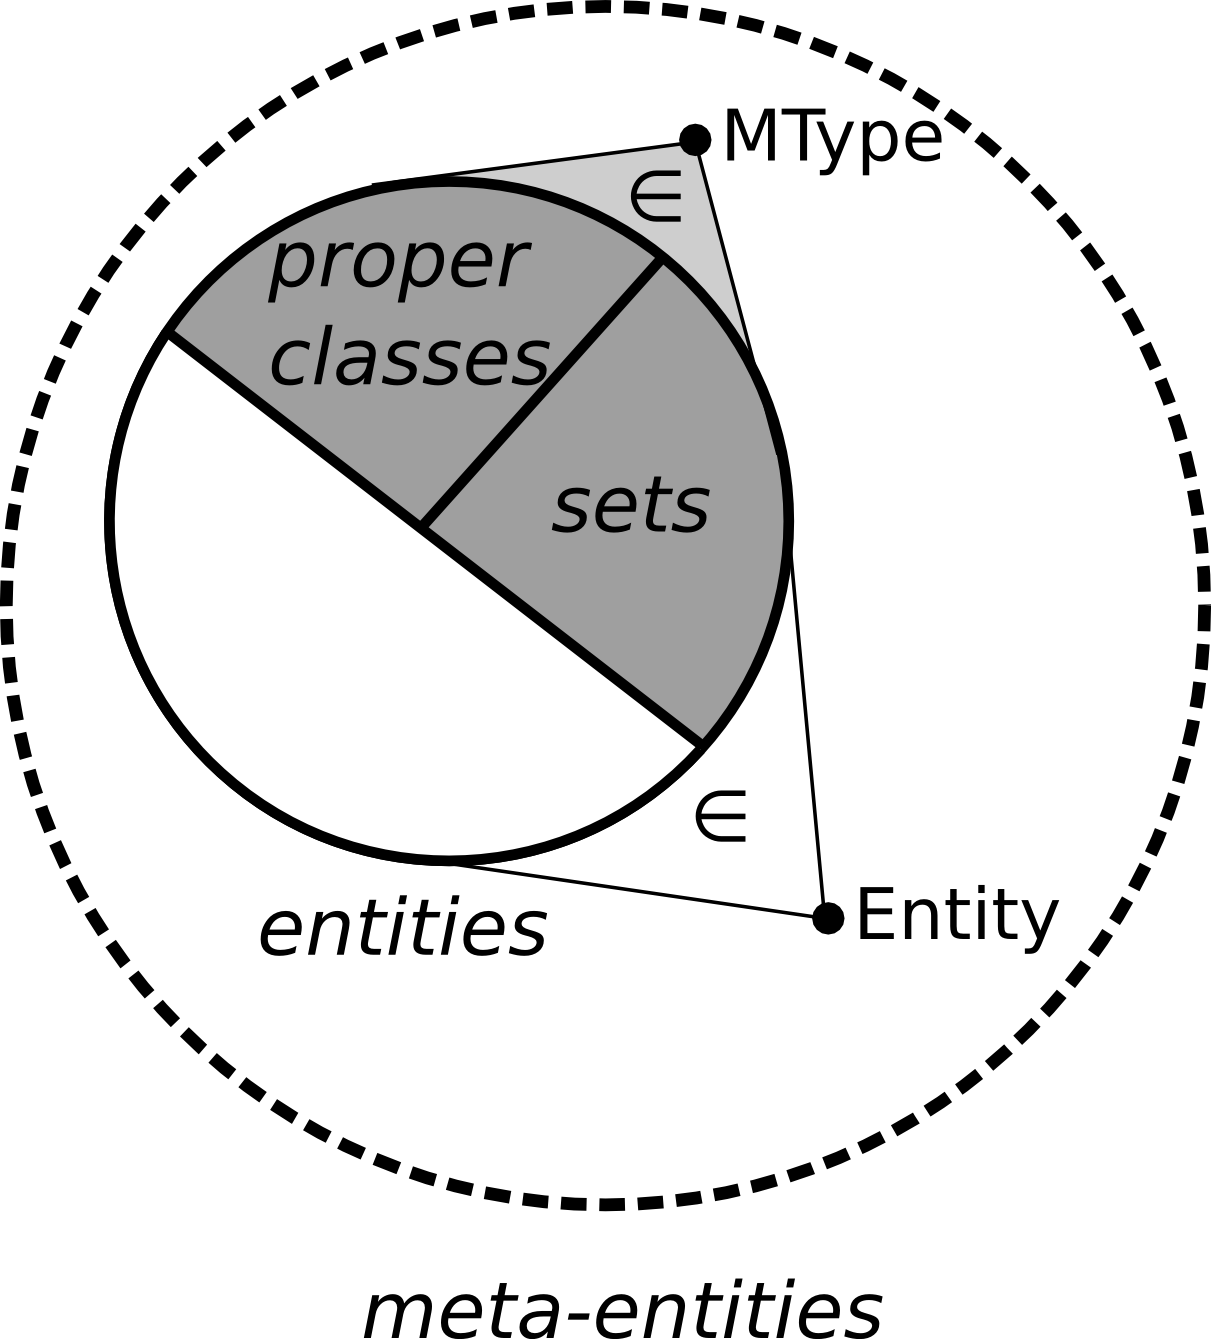
\includegraphics[width=.33\textwidth]{universe}
  \caption{A High-level View of the RESOLVE Mathematical Universe\label{fig:universe}}
\end{figure}

	%---------------------------------------------------------------------
	\subsection{Mechanisms for Static Reasoning\label{staticReasoning}}
	%---------------------------------------------------------------------

		%-------------------------------------------------------------
		\subsubsection{Type Theorems\label{typeTheorems}}
		%-------------------------------------------------------------

\paragraph{Design\label{typeTheoremDesign}}
A practical problem with first-class types is the ability to specify types and type-matching situations that are undecidable.  This is an issue common to all systems that permit dependent types--which a system of truly first-class types must necessarily do.

For example we could imagine two types defined by arbitrary predicates:

\begin{lstlisting}
Definition T1 : MType = {E : MType | P(E)};
Definition T2 : MType = {E : MType | Q(E)};
\end{lstlisting}

Determining whether or not an object modeled by \texttt{T1} can be passed where one modeled by \texttt{T2} is expected is equivalent to asking if $\forall e : $\texttt{MType}$, Q(e) \rightarrow P(e)$, which is, of course, undecidable.

Some verification systems (e.g., Coq) take advantage of this very property as an aid to verification, reducing all programs to reasoning about complex types and casting verification as a type-matching problems.  However, because our goal is to increase the usability of our system by providing the user with strong tool support, we would ideally like to provide the usual static type-safety expected by object-oriented programmers.

In order to provide such static type checking in a variety of useful (but potentially undecideable) situations, we rely on the mathematician to provide and prove explicit type mappings in cases where the reasoning is complicated.

In some cases, relationships can be easily inferred.  For example, the case of simple sub-types:

\begin{lstlisting}
Definition Z : MType = ...;
Definition N : Power(Z) = ...;
\end{lstlisting}

Here we can easily note in the symbol table that an \texttt{N} would be acceptable wherever a \texttt{Z} is required and permit such a shift in conception-of-type in certain well-defined cases.

However, hard-coding such relationships does not provide a general mechanism for reasoning about type relationships and with first-class types, we may quickly arrive in situations where we'd expect the ability to reason about complex type relationships without requiring explicit assertions from the programmer or mathematician.  Consider this application of \texttt{Str}s:

\begin{lstlisting}
Definition Average(S : Str(Z)) : Z = ...;
Definition SomeNs : Str(N) = <1, 10, 3, 19>;
Definition AverageOfSomeNs : Z = Average(SomeNs);
\end{lstlisting}

In an ideal world we would expect this to type-check.  But it is not the case that for two arbitrary type schemas, if the parameters of the one are subtypes of the parameters for the other, then the results are themselves subtypes.  Consider this (somewhat contrived) complement string type:

\begin{lstlisting}
Definition ComplementStr(T : MType) : MType = 
	{S : UntypedStr | For all i, where 0 <= i < |S|,
		Element_At(S, i) not_in T);
\end{lstlisting}

This is the type of all strings containing possibly-heterogenously-typed elements where no element is of type \texttt{T}.  Clearly, \emph{this} set of definitions should \emph{not} typecheck:

\begin{lstlisting}
Definition Average(S : ComplementStr(Z)) : Z = ...;
Definition NotSomeNs : ComplementStr(N) = <-1, -10, -3, -19>;
Definition AverageOfNotSomeNs : Z = Average(SomeNs);
\end{lstlisting}

However, the same thing that got us into this mess---first-class types---provides a road out.  Because types are normal mathematical values and we already have a mechanism for asserting theorems about mathematical values, we can use that existing mechanism to provide information about type relationships.

Because such theorems must take a specific form if they're to be understood by the static type-checker, we add some special syntax, calling them \texttt{Type Theorem}s instead of ordinary \texttt{Theorem}s.  This flags these theorems for the type checker and ensures that we can raise an error if they do not have the proper form.

Such theorems have a number of uses:

\subparagraph{Simple Subtype}
Here is a type theorem stating that, among other things, \texttt{Str(N)}s should be acceptable where \texttt{Str(Z)}s are required:

\begin{lstlisting}
Type Theorem Str_Subtype_Theorem:
	For all T1 : MType, For all T2 : Power(T1),
	For all S : Str(T2),
		S : Str(T1);
\end{lstlisting}

As with any other theorem in the RESOLVE system, this one would require a proof to establish its correctness and maintain soundness.  We assume the presence of a proof-checking subsystem and leave such proofs outside the scope of this research.

\subparagraph{Overlapping Types}
Sometimes, more complex relationships are required.  For example, in some circumstances, providing a \texttt{Z} where an \texttt{N} is expected should be acceptable.  We can use the same mechanism to provide for this case:

\begin{lstlisting}
Type Theorem Z_Superset_of_N:
	For all m : Z, (m >= 0) implies m : N;
\end{lstlisting}

This permits us, under a limited set of circumstances, to provisionally accept a ``sane'' type reassignment, while raising an appropriate proof obligation that the value in question is non-negative.  This is similar to Java, where sane typecasts (i.e., from a \texttt{List} to an \texttt{ArrayList}) are permitted, but cause a run-time check to be compiled into the code.  Here, however, we pay the penalty only once---during verification-time---rather than with each run of the program.

\subparagraph{Complex Expression Type}
We can also use this flexibility to assure the static type-checker that expressions with certain forms have particular types.  For example, we may indicate that, while multiplication generally yields \texttt{Z}s, when one of the factors is from the set of even numbers, \texttt{E}, the result will be as well:

\begin{lstlisting}
Type Theorem Multiplication_By_Even_Also_Even_Right:
	For all i : Z, For all e : E,
		i * e : E;
\end{lstlisting}

Such theorems need no be quantified.  And so, for example, we can use one to resolve a tricky design problem: given that we'd usually like to work with restricted sets that contain only elements of some homogenous type, do we define a separate \texttt{Empty\_Set} for each?  Clearly this is non-intuitive and introduces a number of strange situations.  But type theorems resolves this issue easily.  Given RESOLVE's built-in ``class of all sets'', \texttt{SSet}:

\begin{lstlisting}
Definition Set : MType -> Power(SSet);

Definition Empty_Set : Set;

Type Theorem Empty_Set_In_All_Sets:
	For all T : MType,
	For all S : Set(T),
		Empty_Set : S; 
\end{lstlisting}

We now have a single term, \texttt{Empty\_Set}, that is defined to be a member of the hetergenous \texttt{SSet}, but then stated to be in any restricted \texttt{Set}.

\subparagraph{Modular Relationships}
In addition to the obvious usability this flexibility adds to RESOLVE's mathematical theories, it also support modularity by permitting types to relate to each other only when they are loaded.  A common arrangement in virtually all mathematical systems is to have a ``numerical tower'', in which \texttt{N} is defined in terms of \texttt{Z}, which is in term defined in terms of \texttt{R}, and so forth.

To begin with, this creates complexity for the end user if the numeric tower is not rooted sufficiently deep for their needs.  The system's entire conception of numbers must change as a higher theory is added.  But more importantly for our design, this violates modularity--in order to use \texttt{N}s, I must also import \texttt{Z}s and \texttt{R}s and complex numbers and the rest of the tower.  The user, and more importantly the automated prover, has no idea which body of theorems are practically relevant.

By using type theorems, relationships can be established as needed.  For example, natural number theory need not advertise a relationship to \texttt{Z} (though practically, integers will likely form part of its internal definition details):

\begin{lstlisting}
Definition N : MType;
\end{lstlisting}

However, when \texttt{Integer\_Theory} is loaded, it may then establish its relationship with \texttt{N}:

\begin{lstlisting}
Definition Z: MType,

Type Theorem N_Subset_of_Z:
	For all n : N,
		n : Z;
\end{lstlisting}

This design splits the difference between a rich, expressive type system and the straightforward static typing programmers have come to expect.  Simple cases can be covered without thought on the part of the programmer, while complex, undecidable cases are permitted by explicitely deferring to the prover.

\paragraph{Design\label{typeTheoremImplementation}}

Most of the features listed in this chapter exist in other systems and are novel primarily for being gathered in one place alongside a practical, imperative programming lanaguage.  Type theorems, however, are to our knowledge entirely novel, and we therefore will spend a short amount of time discussing their implementation.

Each type theorem introduces two, possibly three pieces of information: an \emph{expression pattern}, which we seek to bind against the actual value, an \emph{asserted type}, which the pattern is said to inhabit, and, optionally, a \emph{condition}, which the actual value must meet in order for the relationship to hold.  As a practical example, consider:

\begin{lstlisting}
Type Theorem Z_Superset_of_N:
	For all m : Z, (m >= 0) implies m : N;
\end{lstlisting}

Here, the expression pattern is \texttt{m}, the asserted type is \texttt{N}, and the condition is \texttt{(m >= 0)}.  If the condition is omitted, we default it to \texttt{true}.

Each time a new type theorem is accepted, we take the type of the expression pattern and the asserted type and determine their \emph{canonical bucket}, before finding the associated buckets in the type graph and added an edge.

Canonicalization transforms a type that possibly contains free type variables into a Big Union type that contains any valuation of those variables.  This is accomplished by introducing new variables indexed by the Big Union for each type variable (even if the variables are not unique), ranging over \texttt{MType}.

So, if a type started life as $T \cup W \cup T$, where $T$ ranges over \texttt{MType} and $W$ over \texttt{Power(T)}, it would be canonicalized into $\bigcup_{T_1 : MType, T_2 : MType, T_3 : MType} T_1 \cup T_2 \cup T_3$.  Clearly, we have lost a fair bit of information here, but that is attached to the newly added edge in the form of \emph{static requirements}.

In this case, the static requirements would be: $T_1 : MType, T_2 : Power(T_1), T_3 = T_1$.

The expression pattern and condition are also added to the edge.

When we seek to determine if a given value is acceptable in a particular type, we first canonicalize the type of the value, then seek out any canonical buckets that are \emph{syntactic supertypes} of that type, which is a simpler kind of type reasoning based on a short list of hard-coded rules.  We do the same for the expected type.  We then determine if there are edges from any of the provided value's buckets to any of the expected type's buckets.  For each such edge, we iterate, attempting to bind the value to the pattern expression, then use the resulting bindings to satisfy the static requirements, before finally instantiating the condition and adding it to a list.

We continue searching until we find an edge whose condition is simply \texttt{true}, or we run out of edges.  If any edge's condition is \texttt{true}, we simply return true.  If no edge matched, we return \texttt{false}.  In any other case, we return the disjunction of the condition of each matched edge.

%-----------------------------------------------------------------------------
\section{Future Work}
%-----------------------------------------------------------------------------
The design of the new mathematical and specification subsystem has already been completed at a high level, though work remains to formalize it more completely. In particular, while we believe that the addition of higher-order definitions should not pose any soundness problems since uninterpretted definitions eschew many of the problems related with higher-order theories, this requires more research and theory development to establish.  This said, formally establishing the soundness of the new theory is outside the scope of this research---we seek to demonstrate only the usefulness of this level of abstraction; future work may be required to refine the mathematical details.

Uninterpretted, higher-order definitions have been implemented and well-tested.  The framework for the new type system has been laid and is awaiting the implementation of type theorems before it can be fully implemented and tested.  Once in place, first-class types, the MK set theory, and type theorems will be tested together and refined against a set of target mathematical theories that will be designed to start simple and graduate eventually to the level of complication of generic theories of trees.  While the simpler of these theories have already been developed, the higher-level ones remain.

